\documentclass[12pt]{amsbook}
\usepackage{preamble}

\begin{document}
\pagenumbering{gobble} % This kills the page numbering

\begin{center}
   \textsc{\large MATH 272, Exam 1}\\
\end{center}
\vspace{1cm}

\noindent\textbf{Name} \; \underline{\hspace{8cm}}

\vspace{1cm}

\noindent\textbf{Instructions} \; No textbook, homework, calculators, phones, or smart watches may be used for this exam. The exam is designed to take 50 minutes and must be submitted at the end of the class period. All of your solutions should be easily identifiable and supporting work must be shown. You may use any part of this packet as scratch paper, but please clearly label what work you want to be considered for grading. Ambiguous or illegible answers will not be counted as correct.\\

\noindent\emph{Only the highest scoring \underline{five} problems will be counted towards your total score. You cannot get over 75 points.}

\vspace{1cm}

\begin{flushleft}
\textbf{Problem 1} \; \underline{\hspace{1cm}}/15

\vspace{.25cm}

\textbf{Problem 2} \; \underline{\hspace{1cm}}/15

\vspace{.25cm}

\textbf{Problem 3} \; \underline{\hspace{1cm}}/15

\vspace{.25cm}

\textbf{Problem 4} \; \underline{\hspace{1cm}}/15

\vspace{.25cm}

\textbf{Problem 5} \; \underline{\hspace{1cm}}/15

\vspace{.25cm}

\textbf{Problem 6} \; \underline{\hspace{1cm}}/15

\vspace{.5cm}

\textbf{Total} \;\hspace{1.1cm} \underline{\hspace{1.25cm}}/75
\end{flushleft}

\vspace*{4cm}


\begin{center}\large{There are extra pages between each problem for scratch work.\\

Please circle your answers!}\end{center}

\newpage
\begin{center}\large{A table of Fourier transforms and their inverses.} \end{center}
\begin{table}[H]
        \centering
        \renewcommand{\arraystretch}{2}
        \begin{tabular}{c|c}
            $f(x)$ & $\hat{f}(k)$\\
            \hline
         	$\delta(x)$ & $1$\\
         	$1$ & $\delta(k)$\\
         	$e^{iax}$ & $\delta\left(k-\frac{a}{2\pi}\right)$\\
         	$\cos(ax)$ & $\frac{\delta\left(k-\frac{a}{2\pi}\right)+\delta\left(k+\frac{a}{2\pi}\right)}{2}$\\
     		$\sin(ax)$ & $\frac{\delta\left(k-\frac{a}{2\pi}\right)-\delta\left(k+\frac{a}{2\pi}\right)}{2i}$\\
     		$e^{-\alpha x^2}$ & $\sqrt{\frac{\pi}{\alpha}} e^{\frac{(\pi k)^2}{\alpha}}$
        \end{tabular}
        \label{tab:fourier_transform}
    \end{table}
    
   \vspace*{2cm}
\begin{center}\large{Integration by parts:}\end{center}

 	\[
 	\int_a^b udv = \left. uv \right\vert_a^b - \int_a^b vdu.
 	\]







% Problem 1
\newpage
\begin{problem}~\\

\def\arraystretch{2}% increase vertical spacing
\noindent\begin{tabularx}{\textwidth}{cXcc}
 & & T & F\\
(\theabc) & The equation 
\[
-\frac{d^2}{dx^2}f(x) = \delta(x)
\]
where $x\in \R$ has a solution. & \answerbox & \answerbox\\
(\theabc) & A linear operator $\mathcal{L}$ satisfies
\[
\mathcal{L}(f+\alpha g) = \mathcal{L}f + \alpha \mathcal{L}g
\]
for any constant $\alpha$ and functions $f$ and $g$. & \answerbox & \answerbox\\
(\theabc) & A constant function $f(x)=c$ is an eigenfunction of the derivative operator $\mathcal{L}=\frac{d}{dx}$ & \answerbox & \answerbox\\
(\theabc) & The Dirac delta defined on $[0,L]$ cannot be written as a Fourier series. & \answerbox & \answerbox\\
(\theabc) & An inner product $\innprod{\cdot}{\cdot}$ also allows one to define a distance function $d(\cdot,\cdot)$. & \answerbox & \answerbox\\
\end{tabularx}
\end{problem}

\newpage
\emph{Intentionally left blank to be used as scratch paper.}\\


% Problem 2
\newpage
\begin{problem}
\begin{enumerate}[(a)] Consider the function $f\colon [-\pi,\pi] \to \C$ given by $f(x) = x+i\sin(x)$.
	\item (\textbf{5 pts.}) Plot this function in the complex plane below.
		\[
		        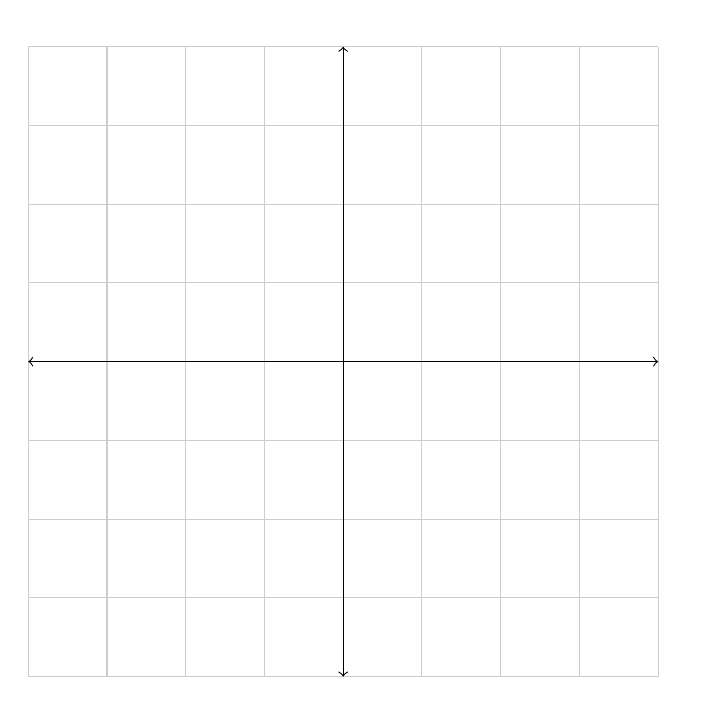
\begin{tikzpicture}[scale=1]
		        \draw[thin,gray!40] (-4,-4) grid (4,4);
		        \draw[<->] (-4,0)--(4,0) node[right]{$\RE$};
		        \draw[<->] (0,-4)--(0,4) node[above]{$\IM$};
		        \end{tikzpicture}
		  \]
	\item (\textbf{5 pts.}) Compute the norm of the function $\|f\|$ using the Hermitian inner product for the interval $[-4,4]$.
	\vspace*{5cm}
	
	\item (\textbf{5 pts.}) Show that the function $g(x)= a+bi$ with $a$ and $b$ real constants is orthogonal to $f(x)$. \emph{Hint: Use the fact that $g(x)$ is constant and $f(x)$ is odd.}
\end{enumerate}
\end{problem}

\newpage
\emph{Intentionally left blank to be used as scratch paper.}\\


% Problem 3
\newpage
\begin{problem} Consider the linear differential equation $-\frac{d^2}{dx^2}f(x)=\omega^2f(x)$ where $\omega$ is a constant. In this problem we seek to understand the premise behind the Fourier transform.
\begin{enumerate}[(a)]
	\item	(\textbf{4 pts.}) Suppose that both $\chi_1(x)$ and $\chi_2(x)$ are solutions. Show that $f(x)=\alpha_1 \chi_1(x)+ \alpha_2 \chi_2(x)$ is also a solution.
	\vspace*{4cm}
	
	\item	(\textbf{4 pts.}) If we have that $\chi_n(x)$ is a solution for all \underline{integers} $n$, show or explain why 
	\[
	f(x) = \sum_{n=-\infty}^\infty  \alpha_n \chi_n(x),
	\]
	is also a solution.
	\vspace*{4cm}
	
	\item	(\textbf{4 pts.}) If indeed $\chi_k(x)$ is a solution for all \underline{real numbers} $k$, show or explain why 
	\[
	f(x) = \int_{-\infty}^\infty \alpha_k \chi_k(x) dk,
	\]
	is also a solution.
	\vspace*{4cm}
	
	\item	(\textbf{3 pts.}) If every function $f(x)$ corresponds to a unique list of coefficients $\alpha_k$, explain why it suffices to manipulate the coefficients $\alpha_k$ to solve a differential equation.
	
\end{enumerate}
\end{problem}

\newpage
\emph{Intentionally left blank to be used as scratch paper.}\\


% Problem 4
\newpage
\begin{problem}
For the following, assume we are using the Hermitian inner product
\[
\innprod{f}{g} = \int_0^L f(x)g^*(x)dx.
\]
Also, assume any functions satisfy $f(0)=f(L)$.
\begin{enumerate}[(a)]
	\item (\textbf{4 pts.}) Let $\hat{a}$ be an operator and $\hat{a}^\dagger$ be the adjoint. Show that the operator $\hat{a}\hat{a}^\dagger$ is Hermitian.
	\vspace*{3cm}
	
	\item (\textbf{4 pts.}) Let $\hat{a} = \frac{d}{dx}$. Show using integration by parts that the adjoint operator is $\hat{a}^\dagger  = -\frac{d}{dx}$.
	\vspace*{4cm}
	
	\item (\textbf{2 pts.}) Is $\hat{a}$ Hermitian?
	\vspace*{3cm}
	
	\item (\textbf{4 pts.}) Explain why the spectrum of the operator $\Delta = - \frac{d^2}{dx^2}$ is real.
	\vspace*{3cm}
	
	\item (\textbf{4 pts.}) Could there be a solution to the equation
	\[
	\Delta f(x) = i f(x)?
	\]
	Explain.
\end{enumerate}
\end{problem}

\newpage
\emph{Intentionally left blank to be used as scratch paper.}\\


% Problem 5
\newpage
\begin{problem} Let $f(x)$ be a function defined on $[0,L]$.  We want to represent $f(x)$ as a Fourier series by
\[
f(x) = a_0 + \sum_{n=1}^\infty a_n \sqrt{2} \cos\left(\frac{2n \pi x}{L}\right) + \sum_{n=1}^\infty b_n \sqrt{2} \sin\left(\frac{2n\pi x}{L}\right).
\]
\begin{enumerate}[(a)]
	\item (\textbf{4 pts.}) How do you compute the coefficient $a_0$?
	\vspace*{4cm}
	
	\item (\textbf{4 pts.}) How do you compute the coefficients $a_n$ and $b_n$?
	\vspace*{4cm}
	
	\item (\textbf{4 pts.}) Explain why the function $f(x) = \frac{1}{x-\frac{L}{2}}$ does not have a Fourier series representation. \emph{Hint: Can you compute the coefficients?}
	\vspace*{4cm}
	
	\item (\textbf{3 pts.}) If a function has a Fourier series, explain why that series representation must be unique. \emph{Hint: Could you possibly get two different answers for the coefficients?}
\end{enumerate}
\end{problem}

\newpage
\emph{Intentionally left blank to be used as scratch paper.}\\


% Problem 6
\newpage
\begin{problem}
The Fourier transform of a function $f(x)$ is given by
\[
\fourier{f(x)}=\int_{-\infty}^\infty f(x) e^{-i2\pi kx}dx = \hat{f}(k).
\]
\begin{enumerate}[(a)]
	\item (\textbf{4 pts.}) Assuming $f(-\infty)=0=f(\infty)$, show using integration by parts that $\fourier{\frac{d}{dx}f(x)} = (i2\pi k) \hat{f}(k).$
	\vspace*{4cm}
	
	\item (\textbf{4 pts.}) Argue why (a) implies that 
	\[
	\fourier{\frac{d^n}{dx^n}f(x)} = (i2\pi k)^n \hat{f}(k).
	\]
	\vspace*{4cm}
	
	\item (\textbf{4 pts.}) Using the table, find the Fourier transform of 
	\[
	g(x) = \sin(\omega x). 
	\]
	\vspace*{4cm}
	
	\item (\textbf{4 pts.}) Using previous results, apply the Fourier transform to the following differential equation.
	\[
	\frac{d^2}{dx^2}f(x) + 2 \frac{d}{dx}f(x) + f(x) = \sin(\omega x).
	\]
\end{enumerate}
\end{problem}
\newpage
\emph{Intentionally left blank to be used as scratch paper.}\\

\end{document}  